\section{Background}
\label{sec:background}

This section discusses data center architectures that are commonly implemented today.  We discuss both network topologies and network stacks.  Of course, we do not claim that all data centers follow these architectures, however, we have found them to be the most common.

\subsection {Network Topology}

Most data center network topologies today follow a hierarchical approach, using two or three levels of hierarchy~\cite{Al-Fares:2008:SCD}.  The edge is the lowest level of hierarchy, and typically consists of a set of servers in a rack connected to a top-of-rack switch.  At the next level, the aggregation level, a set of switches connect all top-of-rack switches together.  The root of the hierarchy, the core level, contains a set of root switches that connect the aggregation level switches together.  

More bandwidth is allocated to switches and links at higher levels of the hierarchy to cope with the larger amount of traffic due to the aggregation of traffic from lower levels.  For example, edge level switches may use 1 GigE links to connect servers in a rack together, while aggregation level switches may use 10 GigE (or multiple 10 GigE links) to connect edge level servers together.  Core level switches may have even higher bandwidth, using either 40 GigE links or multiple 10 GigE links.

We consider two network toplogies commonly used today, conventional hierarchical and fat-tree.  Figure~\ref{fig:common_topos} illustrates the two network topologies.  TODO:Describe differences and discuss pros and cons.

\captionsetup[subfloat]{captionskip=-0.003in}
\begin{figure}
    \centering
    \subfloat[Conventional Hierarchical]
    {
        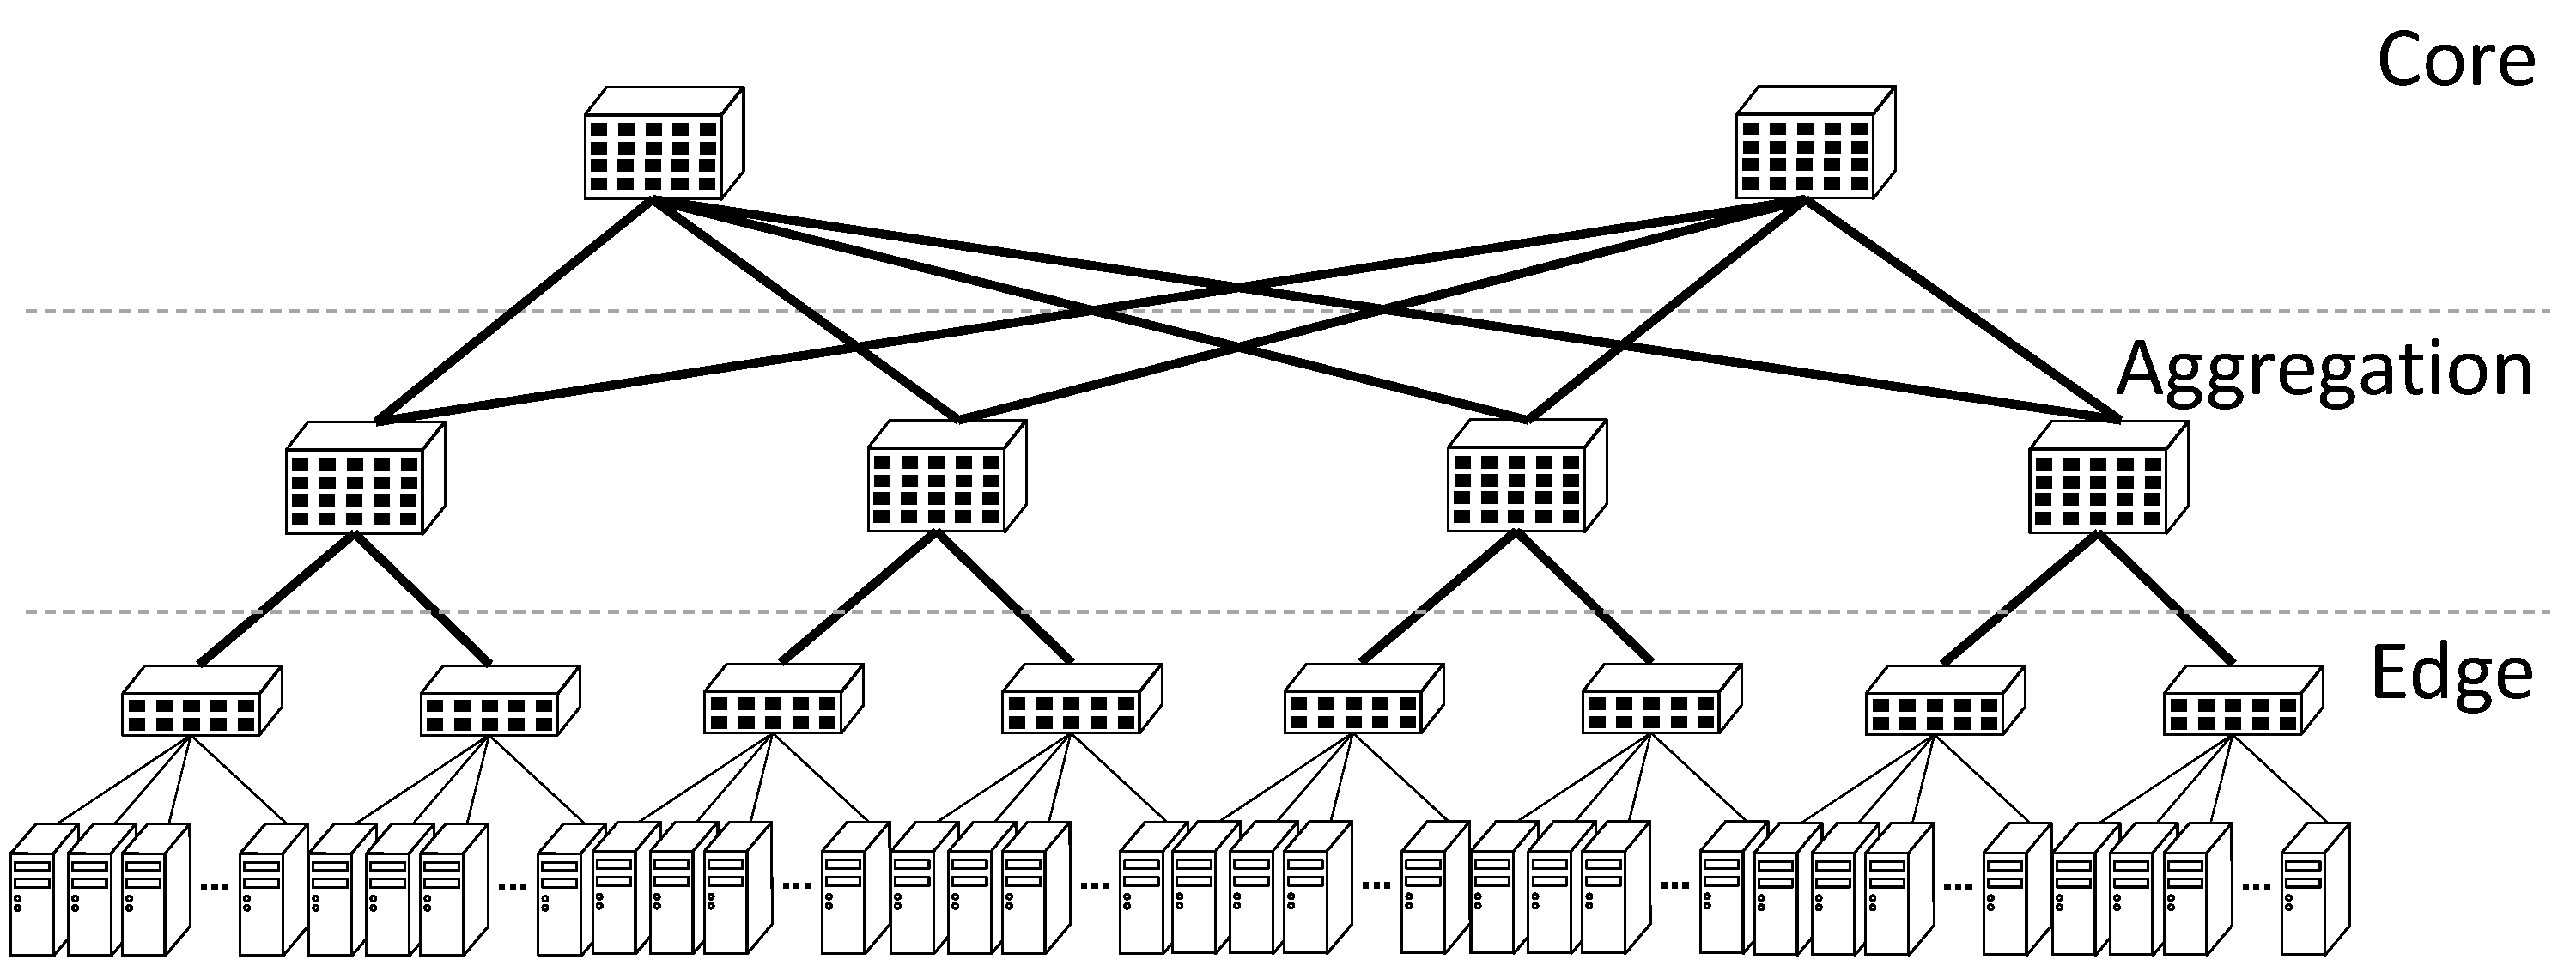
\includegraphics[width=0.5\textwidth]{conventional-hierarchical-topo}
        \label{fig:conventional_hierarchical_topo}
    }
    \\
    \vspace{-0.1in}
    \subfloat[Fat-Tree]
    {
        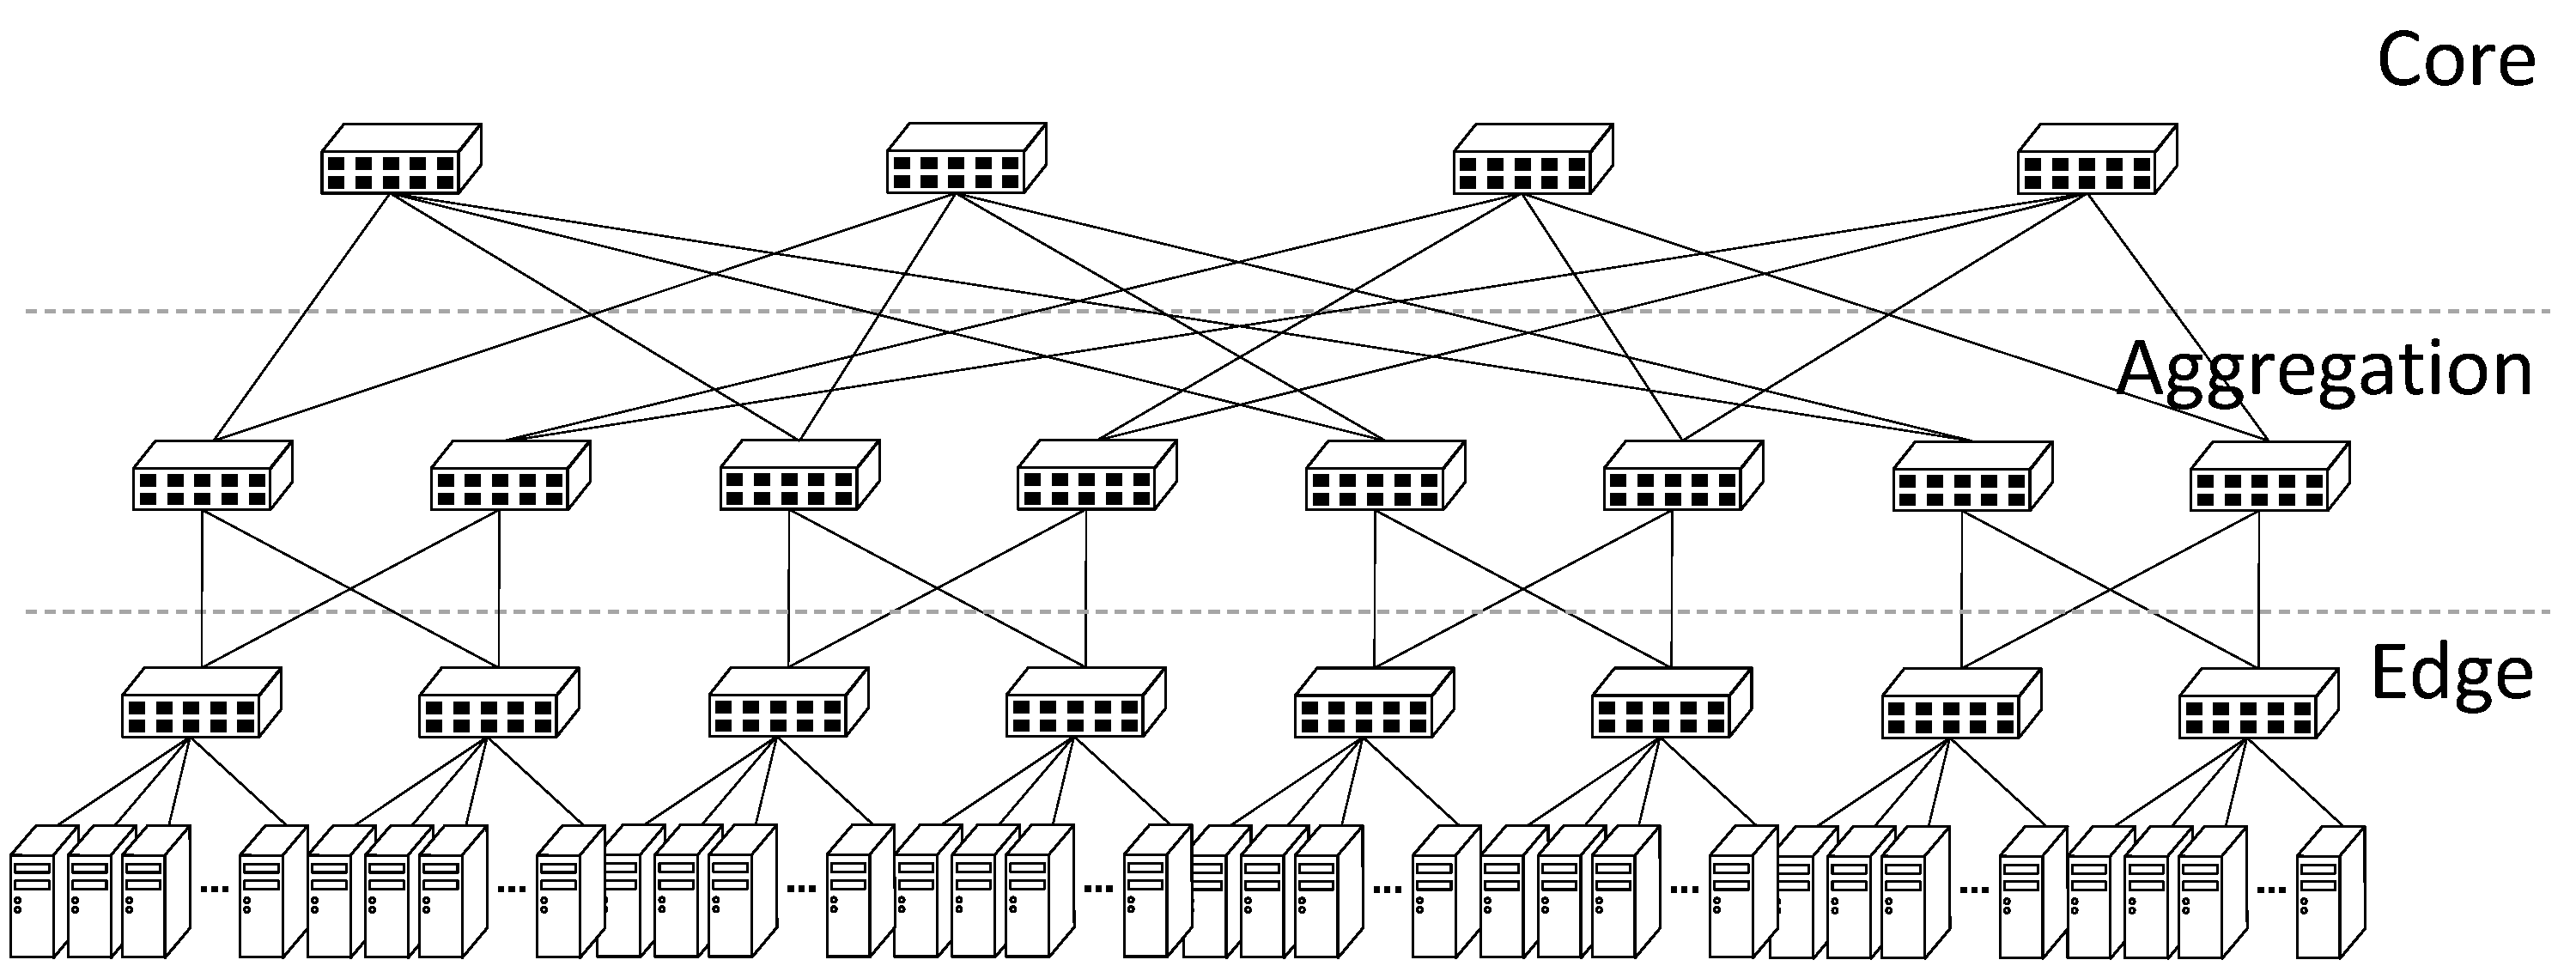
\includegraphics[width=0.5\textwidth]{fat-tree-topo}
        \label{fig:fat_tree_topo}
    }
    \vspace{-0.07in}
    \caption{Common Data Center Network Topologies}
    \label{fig:common_topos}
\end{figure}


\subsection {Network Stack}

Our research has shown that most data centers run a standard Internet stack internally consisting of Ethernet at the link layer, IP at the network layer, TCP or UDP at the transport layer, and a custom application layer protocol.  There may be special cases where proprietary protocols are used internally, however, this is uncommon.
